\chapter{Dataset Details}
\label{app:datasetss}
In \cref{sec:datasetcreation} we detail how our datasets were generated. \Cref{sec:datasetexamples} shows representative examples from each of our datasets.
\section{Dataset Creation}
\subsection{BDD-Inpainting}
\label{sec:datasetcreation}
From the original BDD100K dataset we take a random subset of videos, using 48,886 for a training set and 100 for each held-out test set. Videos are downsampled spatially by a factor of 2.5, center-cropped to $256 \times 256$, and the frame rate is reduced by a factor of three to 10 fps.  We truncate videos to 400 frames, corresponding to a 40 second length for each. We randomly generate a set of 49,970 masks of four types: grids, horizontal or vertical lines, boxes, and blobs. Our mask generation procedure first picks a mask type, and then randomly selects mask parameters such as size and direction of motion (which includes stationary masks). Generated masks contain 400 frames. During training both videos and masks are sampled uniformly and independently, giving a distribution over nearly 2.5 billion video-mask pairs. Our test sets, as well as code for regenerating our training set, will be made public upon publication.

\subsection{Inpainting-Cars}
 We use an in-house dataset of overhead drone footage of vehicle traffic, for which we have tracker-generated bounding boxes for each vehicle. The videos are spatially downsampled by a factor of two from their original 4k resolution, and  $256 \times 256$ sub-videos centred on vehicles are extracted using the vehicle-specific tracks. The length of these videos is variable as it depends on the amount of time a given vehicle was visible in the source video, but typically ranges from 10 to 60 seconds at 10 fps. Bounding boxes are dilated by a factor of two to ensure the entirety of the vehicle is contained within them, and these dilated bounding boxes are then used as masks. This dataset contains 2973 training examples and 100 held-out test examples. 

\subsection{Inpainting-Background}
 The process for creating the Inpainting-Background is nearly identical to that of Inpainting-Cars. The primary difference is that the tracks are shifted in time to find new tracks which do not intersect with the bounding box of any other vehicle, giving a dataset where the masked out region contains the road surface and other environmental factors. Beyond that, videos are processed in the same way and are of the same length as those in Inpainting-Cars. This dataset contains 2965 training examples and 100 held-out test examples.  

 \subsection{Traffic Scenes}
This dataset is created using the same in-house dataset as was used for Inpainting-Cars and Inpainting-Background. The 4k, 10 fps source videos are spatially downsampled by a factor of 7.25, truncated to 200 frames and cropped to $256 \times 256$, with the crops centred over road features like intersections, roundabouts, highway on-ramps, \etc. We generate masks using the same mask generation procedure as in BDD-Inpainting. 
\section{Dataset Examples}
\label{sec:datasetexamples}
\subsection{BDD-Inpainting}
See \cref{fig:bdd-examples} for examples from the BDD-Inpainting dataset. Mask types, shown in green, are indicated for each example.
\begin{figure*}[h!]
\begin{center}
    \centering
    \captionsetup{type=figure}
    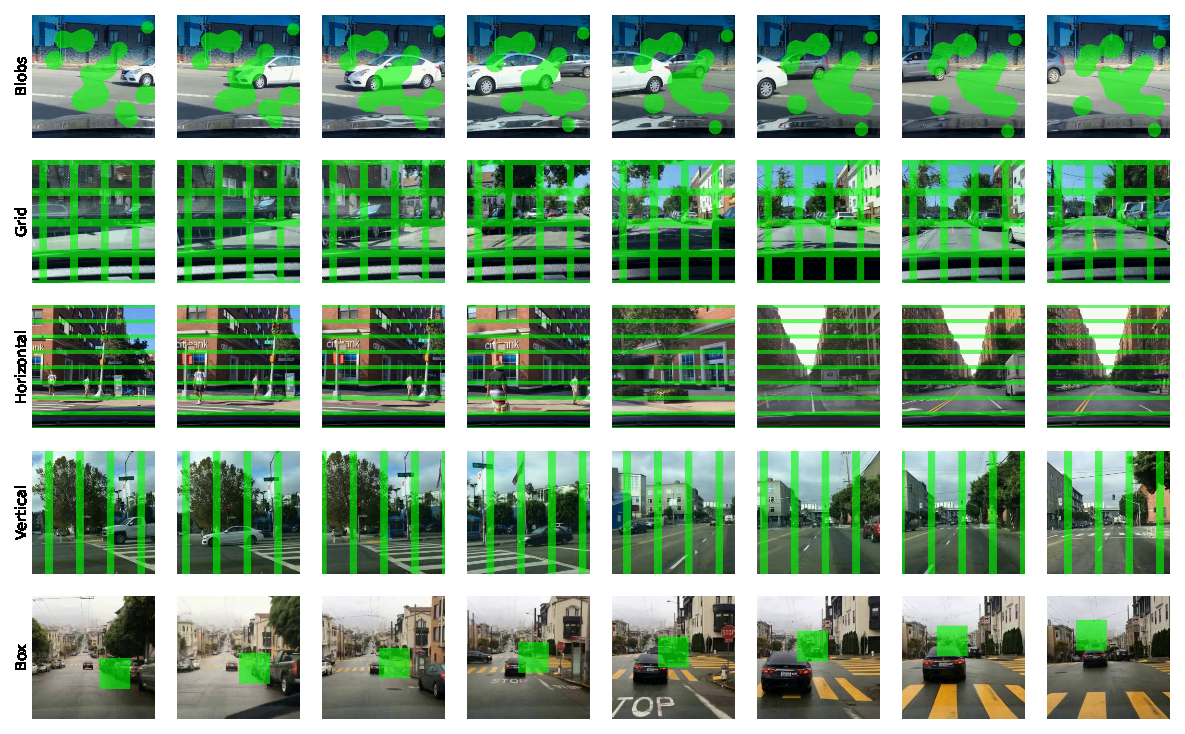
\includegraphics[width=\linewidth]{figures/dataset-examples/bdd-examples.pdf}
    \captionof{figure}{Representative examples from the BDD-Inpainting dataset.}
    \label{fig:bdd-examples}
\end{center}
\end{figure*}
\subsection{Inpainting-Cars}
See \cref{fig:cars-examples} for examples from the Inpainting-Cars dataset. Masks are shown in black.
\begin{figure*}[h!]
\begin{center}
    \centering
    \captionsetup{type=figure}
    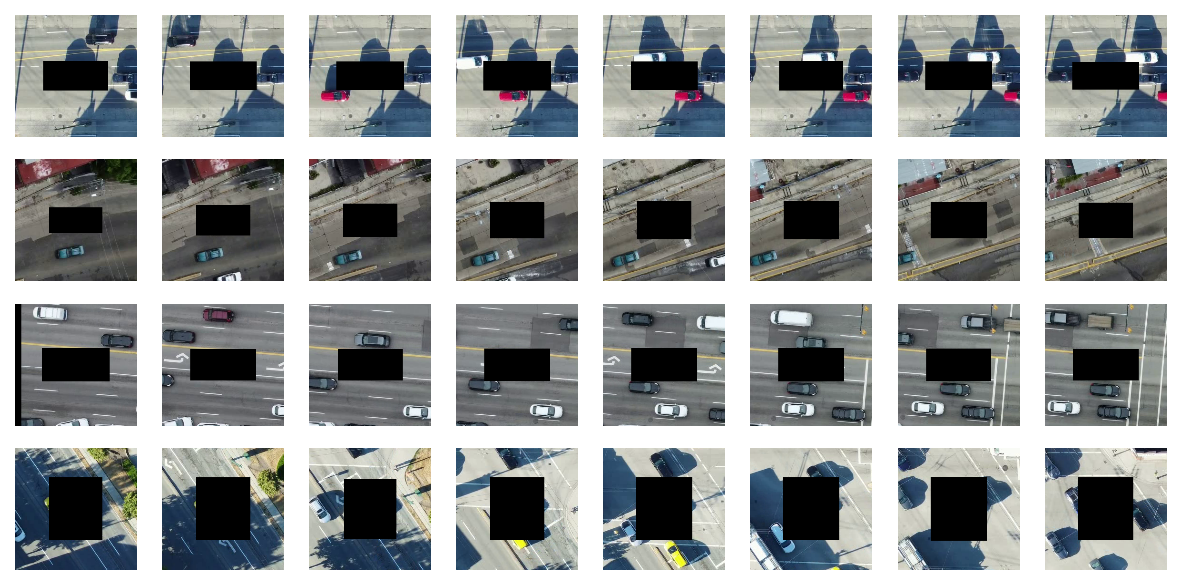
\includegraphics[width=\linewidth]{figures/dataset-examples/cars-examples.pdf}
    \captionof{figure}{Representative examples from the Inpainting-Cars dataset.}
    \label{fig:cars-examples}
\end{center}
\end{figure*}
\subsection{Inpainting-Background}
See \cref{fig:bg-examples} for examples from the Inpainting-Background dataset. Masks are shown in black.
\begin{figure*}[h!]
\begin{center}
    \centering
    \captionsetup{type=figure}
    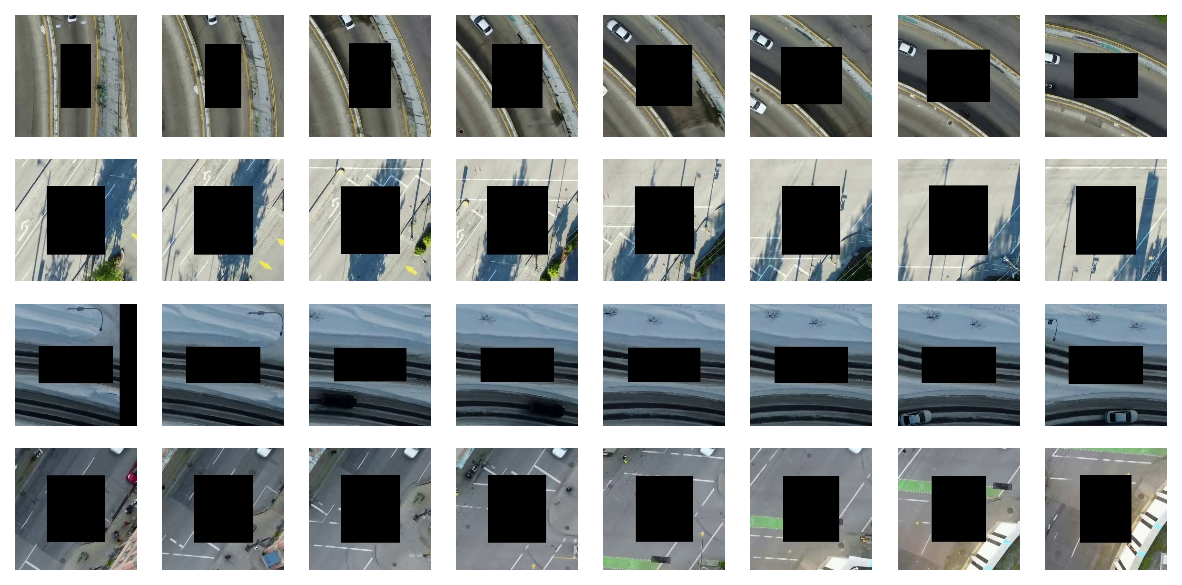
\includegraphics[width=\linewidth]{figures/dataset-examples/bg-examples.pdf}
    \captionof{figure}{Representative examples from the Inpainting-Background dataset.}
    \label{fig:bg-examples}
\end{center}
\end{figure*}
\subsection{Traffic-Scenes}
See \cref{fig:ts-examples} for examples from the BDD-Inpainting dataset. Mask types, shown in green, are indicated for each example.
\begin{figure*}[h!]
\begin{center}
    \centering
    \captionsetup{type=figure}
    \includegraphics[width=\linewidth]{figures/dataset-examples/ts-examples.png}
    \captionof{figure}{Representative examples from the Traffic-Scenes dataset.}
    \label{fig:ts-examples}
\end{center}
\end{figure*}